\chapter{Methods}

This chapter will outline the methods how SCVAEs and non-conditioned VAEs are integrated using multitask learning in this thesis. Initially, describe the method of merging SCVAEs with non-conditioned VAEs by expanding the SCVAEs framework with a second decoder. This method will be applied to both Gaussian VAEs and VQ-VAEs. In the following section, I will describe another method of merging SCVAEs with non-conditioned VAEs by utilizing the same encoder and decoder for both models by employing novel training strategies. This method will also be applied to both Gaussian VAEs and VQ-VAEs.

\section{Method 1: Expanding the VAEs framework}

In the first method, we expand the VAEs framework with a second decoder $p_\xi(x|z,m)$, which is conditioned on an additional property $m$ of the input data. This approach involves utilizing two decoders within the VAEs framework: one for reconstructing the input data solely based on the latent variable $z$, and the other for reconstructing the input data based on both the latent variable $z$ and the additional conditioning information $m$.

\subsection{Conditioning information}

In this method, the conditioning information $m$ is acquired by sampling constant number of pixels from the input data. To sample the pixels from the input image $x$, we will use the sampling operation, which will be described in the following section.

\subsubsection{Sampling operation}

To acquire the conditioning information $m$ from the input image $x$, we will use sampling operation. I will explore two sampling types for this method, which can be seen in Figure~\ref{SamplingFigure} and are described as follows: 

\begin{enumerate}
    \item \textbf{Exact same sampling:} In this sampling type, the conditioning information $m$ is sampled from the input image $x$ by sampling the exact same sparse pixels from the input image $x$. In this work, the pixels that will be sampled from the input image will be a sparse grid of pixels.
    \item \textbf{Uniform random sampling:} In this sampling type, the conditioning information $m$ is sampled from the input image $x$ by sampling exact number of pixels from the input image $x$ uniformly at random.
\end{enumerate}

\begin{figure}[H]
    \centering 
    

\tikzset{every picture/.style={line width=0.75pt}} %set default line width to 0.75pt        

\begin{tikzpicture}[x=0.75pt,y=0.75pt,yscale=-1,xscale=1]
%uncomment if require: \path (0,374); %set diagram left start at 0, and has height of 374

%Image [id:dp9293884018723756] 
\draw (365.67,295.2) node  {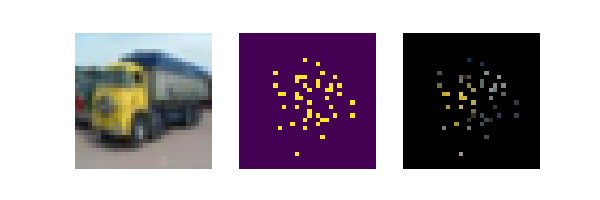
\includegraphics[width=225pt,height=75pt]{figures/assets/GAUSSIAN.png}};
%Image [id:dp548757972749888] 
\draw (365.67,208.8) node  {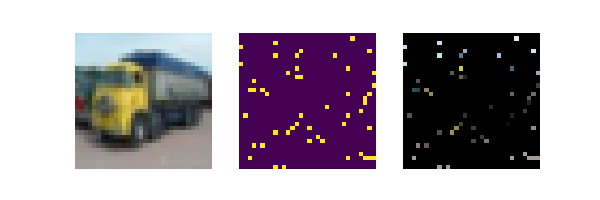
\includegraphics[width=225pt,height=75pt]{figures/assets/UNIFORM.png}};
%Image [id:dp620494998311241] 
\draw (365.67,124.8) node  {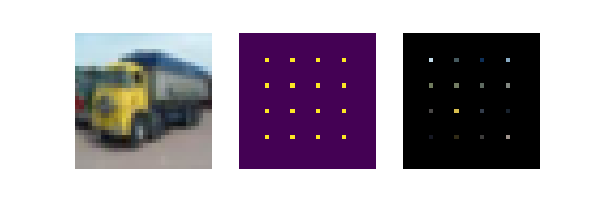
\includegraphics[width=225pt,height=75pt]{figures/assets/EXACT.png}};
%Shape: Grid [id:dp3074430629490833] 
\draw  [draw opacity=0] (242.67,82.33) -- (497.67,82.33) -- (497.67,337.67) -- (242.67,337.67) -- cycle ; \draw   (242.67,82.33) -- (242.67,337.67)(327.67,82.33) -- (327.67,337.67)(412.67,82.33) -- (412.67,337.67)(497.67,82.33) -- (497.67,337.67) ; \draw   (242.67,82.33) -- (497.67,82.33)(242.67,167.33) -- (497.67,167.33)(242.67,252.33) -- (497.67,252.33)(242.67,337.33) -- (497.67,337.33) ; \draw    ;

% Text Node
\draw (279.26,61.29) node [anchor=north west][inner sep=0.75pt]  [rotate=-308.3] [align=left] {original};
% Text Node
\draw (172.67,120) node [anchor=north west][inner sep=0.75pt]   [align=left] {Exact};
% Text Node
\draw (359.26,61.29) node [anchor=north west][inner sep=0.75pt]  [rotate=-308.3] [align=left] {original};
% Text Node
\draw (437.53,61.29) node [anchor=north west][inner sep=0.75pt]  [rotate=-308.3] [align=left] {original};
% Text Node
\draw (165.17,204) node [anchor=north west][inner sep=0.75pt]   [align=left] {Uniform};
% Text Node
\draw (160.17,291) node [anchor=north west][inner sep=0.75pt]   [align=left] {Gaussian};


\end{tikzpicture}

    \caption[Sampling types.]%
    { 
        Sampling types. The first sampling type is to sample the conditioning information $m$ from the input image $x$ by sampling the exact same sparse pixels from the input image $x$. The second sampling type is to sample the conditioned information $m$ from the input image $x$ by sampling number of pixels from the input image $x$ uniformly at random. 
    }\label{SamplingFigure}
\end{figure}

\subsection{Application to Gaussian VAEs}

\begin{figure}[H]
    \centering 
    \centering
\scriptsize
\begin{tabular}{||c|c|c|c||}
\hline
 Method & Parameters & Reconstruction loss & KL loss \\
\hline
\textit{Baseline} & - & 0.0042 +- 1.2e-03 & 0.0018 +- 6.3e-04 \\
\hline
Multi Decoder & Exact sampling & 0.0036 +- 8.3e-04  $\downarrow$ & 0.0027 +- 8.7e-04  $\uparrow$ \\
\hline
Multi Decoder & Exact sampling, SoftAdapt & 0.0034 +- 1.9e-04  $\downarrow$ & 0.0029 +- 2.8e-03  $\uparrow$ \\
\hline
Multi Decoder & Uniform sampling & 0.0035 +- 6.5e-04  $\downarrow$ & 0.0026 +- 1.7e-03  $\uparrow$ \\
\hline
Multi Decoder & Uniform sampling, SoftAdapt & 0.0034 +- 7.3e-03  $\downarrow$ & 0.0029 +- 2.0e-02  $\uparrow$ \\
\hline
\end{tabular}

    \caption[Method 1 applied to Gaussian VAEs.]%
    { 
        Method 1 applied to Gaussian VAEs. The Gaussian VAEs framework is extended by adding a second decoder $p_\xi(x|z,m)$, where $m$ is the conditioned information about the input data. Same as in 

        
        
        
        The input $x$ is passed through the encoder with parameters $\phi$ producing the mean $\mu$ and the standard deviation $\sigma$ of the Gaussian distribution. The random variable $\epsilon$ is sampled from a standard Gaussian distribution and is used to sample $ z = \mu + \sigma \odot \epsilon$. Then the sampled $z$ is used as input to both decoders. The first decoder with parameters $\theta$ produces the output $\hat{x}$. The second decoder with parameters $\xi$ produces the output $\hat{x}$. The loss function to be minimized is the sum of the MSE reconstruction loss and the KL divergence regularization loss.
        
        
        The sampled $z$ is then passed through the decoder with parameters $\theta$ producing the output $\hat{x}$. The loss function to be minimized is the sum of the MSE reconstruction loss and the KL divergence regularization loss. 
    }\label{SCVAE1DFigure}
\end{figure}

\subsection{Application to VQ-VAEs}

\begin{figure}[H]
    \centering 
    \centering
\scriptsize
\begin{tabular}{||c|c|c|c||}
\hline
 Method & Parameters & Reconstruction loss & VQ loss \\
\hline
\textit{Baseline} & - & 0.0022 +- 7.4e-08 & 0.0029 +- 4.1e-07 \\
\hline
Multi Decoder & Exact sampling & 0.0017 +- 6.9e-09  $\downarrow$ & 0.0039 +- 9.8e-07  $\uparrow$ \\
\hline
Multi Decoder & Exact sampling, SoftAdapt & \textbf{0.0013 +- 2.4e-09}  $\downarrow$ & \textbf{0.0016 +- 6.8e-08}  $\downarrow$ \\
\hline
Multi Decoder & Uniform sampling & 0.0018 +- 1.3e-07  $\downarrow$ & 0.0036 +- 3.5e-07  $\uparrow$ \\
\hline
Multi Decoder & Uniform sampling, SoftAdapt & \textbf{0.0017 +- 6.6e-08}  $\downarrow$ & \textbf{0.0021 +- 3.1e-07}  $\downarrow$ \\
\hline
\end{tabular}

    \caption[Architecture of SCVAE1D.]%
    { 
        Architecture of Gaussian VAEs. The input $x$ is passed through the encoder with parameters $\phi$ producing the mean $\mu$ and the standard deviation $\sigma$ of the Gaussian distribution. The random variable $\epsilon$ is sampled from a standard Gaussian distribution and is used to sample $ z = \mu + \sigma \odot \epsilon$. The sampled $z$ is then passed through the decoder with parameters $\theta$ producing the output $\hat{x}$. The loss function to be minimized is the sum of the MSE reconstruction loss and the KL divergence regularization loss. 
    }\label{SCVQVAE1DFigure}
\end{figure}

\section{Method 2}


The first decoder is used to reconstruct the input data, given some conditioned information $m$ about the input data and the latent variable. The second decoder is used to reconstruct the input data with just the latent variable $z$.

and the second decoder is used to reconstruct the input data, given no information about the input data. In this thesis we will explore how we can use sparse pixels from the input data as the information that 

The SCVAE1D method and its VQ-VAE counterpart SCVQVAE1D is 





